\chapter{Architetture con Parallelismo a Livello di Istruzioni}

\section{Architettura della CPU pipeline}

Il concetto alla base di quest'architettura è la parallelizzazione della CPU mediante la \textit{parallelizzazione dell'interprete firmware} delle istruzioni, eseguite dal processore con la collaborazione delle altre unità della CPU stessa.\
È noto che tale interprete costa di più fasi, alcune delle quali eventualmente effettuate in uno stesso ciclo di clock da parte di un processore elementare:

\begin{enumerate}
    \item chiamata istruzione, contenente la lettura dell'istruzione dalla memoria con la cooperazione di MMU e memoria,
    \item decodifica dell'istruzione, preparazione degli indirizzi di eventuali operandi in memoria, preparazione degli eventuali operandi presenti in registri generali,
    \item eventuale lettura degli operandi in memoria, ancora con la cooperazione di MMU e memoria,
    \item fase di esecuzione vera e propria e aggiornamento del contatore istruzioni,
    \item eventuale scrittura dei risultati nei registri generali o in memoria, con la cooperazione di MMU e memoria,
    \item trattamento delle interruzioni.
\end{enumerate}

\noindent Queste fasi hanno un ordinamento totale e operano concettualmente su uno \textit{stream} d'istruzioni:\ di conseguenza l'interprete si presta a una parallelizzazione in \textit{pipeline}.

\subsection{Memoria e MMU}

La fase 1 e la fase 3 (5) necessitano, per essere eseguite in parallelo su istruzioni diversa, di due unità di memoria distinte, una dedicata a memorizzare solo istruzioni (\textit{Memoria Istruzioni}, \textbf{IM}) e l'altra a memorizzare solo dati (\textit{Memoria Dati}, \textbf{DM}).\
Entrambe sono dotate di propria MMU.

IM e DM sono partizioni disgiunte della \textit{cache primaria}.

L'unità MINF (\textbf{Memory Interface}) mette in comunicazione, e arbitra, le richieste per il trasferimento di blocchi nei confronti del livello superiore della memoria esterna.

Il Bus di I/O è connesso alla $\mathrm{MMU}_D$, principalmente allo scopo di implementare la tecnica del Memory Mapped I/O.

\textit{Per non introdurre comunicazioni a domanda-risposta} con il processore nella chiamata dell'istruzione, deleghiamo a IM il compito di leggere, senza soluzione di continuità, istruzioni a indirizzi logici consecutivi, generando di fatto lo \textbf{\textit{stream d'ingresso}} della pipeline.\
A tale scopo, MMUI contiene una copia (IC1) del contatore istruzioni (IC) del processore.

I contenuti di $\mathrm{IC}_1$ e IC sono identici e consistenti \textit{finché} non è eseguita un'istruzione di salto che fa effettivamente saltare, dopodiché verrà ripristinato il nuovo stato consistente.

\subsection{Processore}

Lo stream d'istruzione viene raccolto dallo stadio che chiameremo \textit{Unità Istruzioni} (\textbf{IU}), delegato alle fasi 2, parte della 4 e 6.\
IU \textit{decodifica} ogni istruzione e delega ad altri stadi della pipeline il suo proseguimento.

IU contiene la copia ``affidabile'' del \textit{contatore istruzioni IC}.\
Di conseguenza, è naturale pensare che tutte le \textbf{\textit{istruzioni di salto}} siano eseguite interamente da IU.\
In caso di salto, è assolutamente necessario introdurre una prima \textit{retroazione nella pipeline}, che quindi ``non è una pipeline pura'':\ IU invia l'indirizzo logico di salto a IM che \textit{aggiorna IC1 e lo stream di istruzioni riprende a partire dal nuovo indirizzo}.\
È inevitabile che, in caso di salto, IM possa aver già inviato a IU una o più istruzioni, che quindi dovranno essere scartate finché IU non riceve l'istruzione che ha richiesto esplicitamente.\
Questo fenomeno introduce una prima \textit{degradazione} delle prestazioni.

Inoltre, IU provvede a \textit{calcolare gli indirizzi di memoria} delle \texttt{Load} e \texttt{Store} e a chiedere a DM l'esecuzione delle rispettive operazioni di lettura e scrittura.\
Nel caso di \texttt{Load}, il valore letto verrà inviato da DM a uno stadio successivo della pipeline (EU), nel caso di Store IU provvederà anche a inviare a DM il dato da scrivere.\
Di conseguenza, la \texttt{Store} \textit{termina nella DM}.

Poiché il contatore istruzioni è contenuto in IU, quest'ultima è collegata a UNINT e provvede ad effettuare il \textit{trattamento delle interruzioni}.

Tutte le \textit{istruzioni aritmetico-logiche} sono delegate allo stadio chiamato Unità Esecutiva (EU), che provvede a scrivere il risultato nel registro generale destinazione (fasi 4, 5).\
La \texttt{Load} è vista come un'istruzione ``identità'' con un operando in memoria, ragione per cui è EU a occuparsi di ricevere il dato in memoria e a scriverlo nel registro destinazione.

Tutte le comunicazioni tra unità della pipeline avvengono su collegamenti dedicati con protocollo asincrono.

Occupiamoci ora dei Registri Generali.\
Una soluzione efficiente consiste nel tenerne una doppia copia:\ una in IU ($\mathrm{RG}_1$) e l'altra in EU (RG).\
IU necessità solo di \textit{leggere} i registri generali di $\mathrm{RG}_1$.\
Le modifiche dei registri generali, in istruzioni aritmetico-logiche e di \texttt{Load}, sono effettuate da EU su RG e sono, da quest'unità, comunicate a IU che provvede a scrivere i valori ricevuti in $\mathrm{RG}_1$.\
Di conseguenza, la copia sempre aggiornata è quella in EU (RG), mentre ci saranno dei momenti in cui la copia in IU ($\mathrm{RG}_1$) non sarà aggiornata:\ un meccanismo di sincronizzazione provvede al corretto funzionamento di IU, in particolare a impedire a IU la lettura di registri non ancora aggiornati.

Oltre alla \textit{retroazione dovuta alla presenzadi istruzioni di salto}, un'altra seria causa di retroazione è data dalle \textbf{\textit{dipendenze logiche sui registri generali}}:\ IU può voler leggere in $\mathrm{RG}_1$ il contenuto di un registro che deve ancora essere aggiornato dall'esecuzione in EU di un'istruzione precedente dello stream.\
Entrambe le retroazioni

\begin{itemize}
    \item richiedono che, per ragioni di correttezza, vengano introdotti degli opportuni meccanismi di sincronizzazione che ordinino gli eventi in modo consistente con la semantica del programma,
    \item rappresentano cause di degradazione delle prestazioni.
\end{itemize}

\section{Architettura pipeline astratta}

Adotteremo una visione semplificata dell'architettura, che rappresenta l'\textbf{\textit{ar\-chitettura astratta}}:\ questa è costituita da soli quattro stadi, \textbf{IM}, \textbf{IU}, \textbf{DM}, \textbf{EU}.

\begin{itemize}
    \item Sappiamo sia IM sia DM possono essere realizzati come pipeline di 2 o 3 stadi; si tratta di strutture pipeline ``pure'', che non introducono alcun problema di retroazione o dipendenza locica.\ Considerare sia IM sia DM come un unico sottosistema, avente il tempo di servizio effettivo uguale a quello della scrittura interna, semplifica la valutazione delle prestazioni senza nascondere eventi significativi o introdurre approssimazioni;
    \item come in precedenza, supporremo che il registro IC sia presente in doppia copia in IU e IM e che i registri generali siano presenti in doppia copia in IU ed EU.\ In entrambi i casi, opportuni meccanismi di sincronizzazione assicurano la correttezza di funzionamento quando si verifichino momentanee inconsistenze.
\end{itemize}

\noindent L'architettura astratta ha inoltre le seguenti caratteristiche:

\begin{itemize}
    \item \textit{ogni stadio (sottosistema) ha \textbf{tempo di servizio ideale per istruzione}}: \[t= T_{id}= 2\tau\]
    \item \textit{tutti i canali di comunicazione sono asincroni con grado di asincronia uguale a uno}.
\end{itemize}

\section{Implementazione delle unità della CPU pipeline}

Risolviamo anzitutto il problema della \textit{sincronizzazione tra IU e IM in seguito a istruzioni di salto}.\
La richiesta da IU a IM è accompagnata da un \textit{identificatore unico}, che IM associa all'istruzione inviata a IU, mantenendo lo stesso valore dell'identificatore in tutte le successive richieste finché IU non effettua una nuova richiesta.\
A ogni ricezione di istruzione, IU confronta il proprio valore dell'identificatore con quello ricevuto:\ in caso di concordanza l'istruzione è valida, altrimenti IU scarta l'istruzione ricevuta e attende altre istruzioni finché non trova concordanza.

\subsection{Registri generali}

La sincronizzazione per il corretto uso dei registri generali $\mathrm{RG}_1$ può essere così implementata all'interno dell'unità IU:

\begin{itemize}
    \item a ogni registro $\mathrm{RG}_1$ è associato un \textit{semaforo interno}, non negativo, inizializzato a zero;
    \item per ogni istruzione aritmetico-logica o di \texttt{Load}, IU incrementa di uno il semaforo associato al registro destinazione in $\mathrm{RG}_1$;
    \item ogni volta che scrive in un registro di $\mathrm{RG}_1$ su richiesta di EU, IU decrementa di uno il semaforo associato;
    \item quando IU intende leggere un registro di $\mathrm{RG}_1$ la lettura può avere luogo solo se il semaforo associato al registro stesso è uguale a zero; in caso contrario, IU:
          \begin{enumerate}
              \item si mette in attesa degli aggiornamenti del valore del registro, finché il semaforo non ritorna a zero
                    \begin{center}
                        oppure
                    \end{center}
              \item ricorda la situazione dell'istruzione corrente e continua a servire nuove istruzioni in arrivo.
          \end{enumerate}
\end{itemize}

\subsection{Funzionamento in-order e out-of-order}

Consideriamo le due situazioni 1), 2) descritte a proposito dell'attesa che un registro generale divenga aggiornato.

Il funzionamento 1) non introduce modifiche all'ordinamento delle istruzioni elaborate in IU rispetto allo stream d'ingresso.\
Le architetture che adottano questo funzionamento sono dette ``\textbf{in-order}''.

Il funzionamento 2) introduce modifiche all'ordinamento delle istruzioni elaborate dalla IU rispetto allo stream d'ingresso:\ alcune istruzioni, purché abilitate (tutti i registri utili a IU sono aggiornati), ``scavalcano'' altre istruzioni in attesa.\
Le architetture che adottano questo funzionamento sono dette ``\textbf{out-of-order}''.

\section{Ottimizzazioni}

Avendo individuato le cause di degradazione delle performance, le ottimizzazioni tendenti a ridurne l'effetto devono occuparsi di:
\begin{itemize}
    \item \textit{per le degradazioni dovute ai salti}:
          \begin{itemize}
              \item ridurre la probabilità di salto;
              \item sfruttare i tempi morti, introdotti dalle bolle, per effettuare lavoro utile;
              \item ``predire'' l'esito di salti condizionati in macchine ``out-of-order'';
          \end{itemize}
    \item \textit{per le degradazioni dovute alle dipendenze logiche}:
          \begin{itemize}
              \item ridurre la probabilità di dipendenza logica;
              \item aumentare la distanza delle dipendenze logiche.
          \end{itemize}
\end{itemize}

\subsection{Minimizzazioni delle degradazioni dovute ai salti}

Ciò significa ridurre la frequenza stessa con cui vengono utilizzate istruzioni di salto.\
Si tratta di tipiche ottimizzazioni \textit{a tempo di compilazione}, come:

\begin{itemize}
    \item espansione di \textit{macro}, al posto di subroutine o procedure,
    \item \textit{loop unfolding},
\end{itemize}

\noindent che comportano un aumento della memoria \textit{logica} del processo.\
In termini di memoria \textit{fisica}, queste tecniche possono comportare un aumento del working set del processo.

Un'interessante tecnica a tempo di compilazione è quella chiamata \textit{Delayed Branch}, che può essere considerata un caso particolare di \textit{spostamento di codice}, cioè basata sul concetto di cercare di sfruttare i tempi morti, introdotti dalle potenziali bolle, per effettuare invece lavoro utile.

\subsection{Minimizzazione delle degradazioni dovute alle dipendenze logiche}

A tempo di compilazione possono essere applicate tecniche dirette ad ``allontanare'' il più possibile le istruzioni che sono legate da dipendenze logiche.\
Questo comporta, principalmente, l'adozione di tecniche di \textit{spostamento di codice}.

\subsection{Unità Esecutiva parallela}

L'Unità Esecutiva può essere definita secondo lo schema seguente, contenente:

\begin{itemize}
    \item una Unità Funzionale pipeline \textit{moltiplicatore}/\textit{divisore} in virgola fissa,
    \item una Unità Funzionale pipeline \textit{addizionatore} in virgola mobile,
    \item una Unità Funzionale pipeline \textit{moltiplicatore}/\textit{divisore in virgola mobile}, che può anche includere altre operazioni in virgola mobile, come la radice quadrata,
    \item l'unità \textit{EU\textsubscript{MASTER}}.
\end{itemize}

\noindent L'unità indicata con $\mathit{EU_{MASTER}}$ interfaccia IU e DM e \textit{contiene la copia principale dei registri generali} (\textit{RG}) \textit{e dei registri in virgola mobile RF}.\
Ricevendo una istruzione da IU, il funzionamento è il seguente:

\begin{itemize}
    \item se l'operazione richiesta da IU è una aritmetica corta o una {\ttfamily LOAD}, la \textit{esegue direttamente} (per la {\ttfamily LOAD} attende il dato da DM) e invia a IU il valore del registro generale destinazione e il suo indirizzo;
    \item se l'operazione è lunga in virgola fissa, oppure è in virgola mobile, la distribuisce all'Unità Funzionale corrispondente \textit{insieme ai valori degli operandi} letti dai registri RG o RF rispettivamente.
\end{itemize}

\begin{figure}[H]
    \centering
    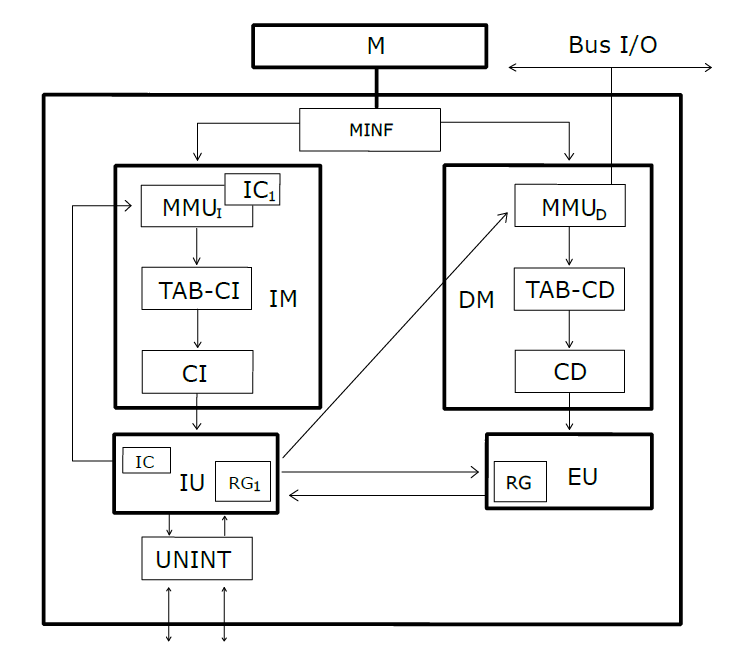
\includegraphics[width=\textwidth]{immagini/Architettura_pipeline.png}
\end{figure}
